\section{Results}
\subsection{Ordinary Least Squares Regression on Franke Function data}
\begin{figure}[h]
    %\centering
    %\hspace{-2.8cm}
    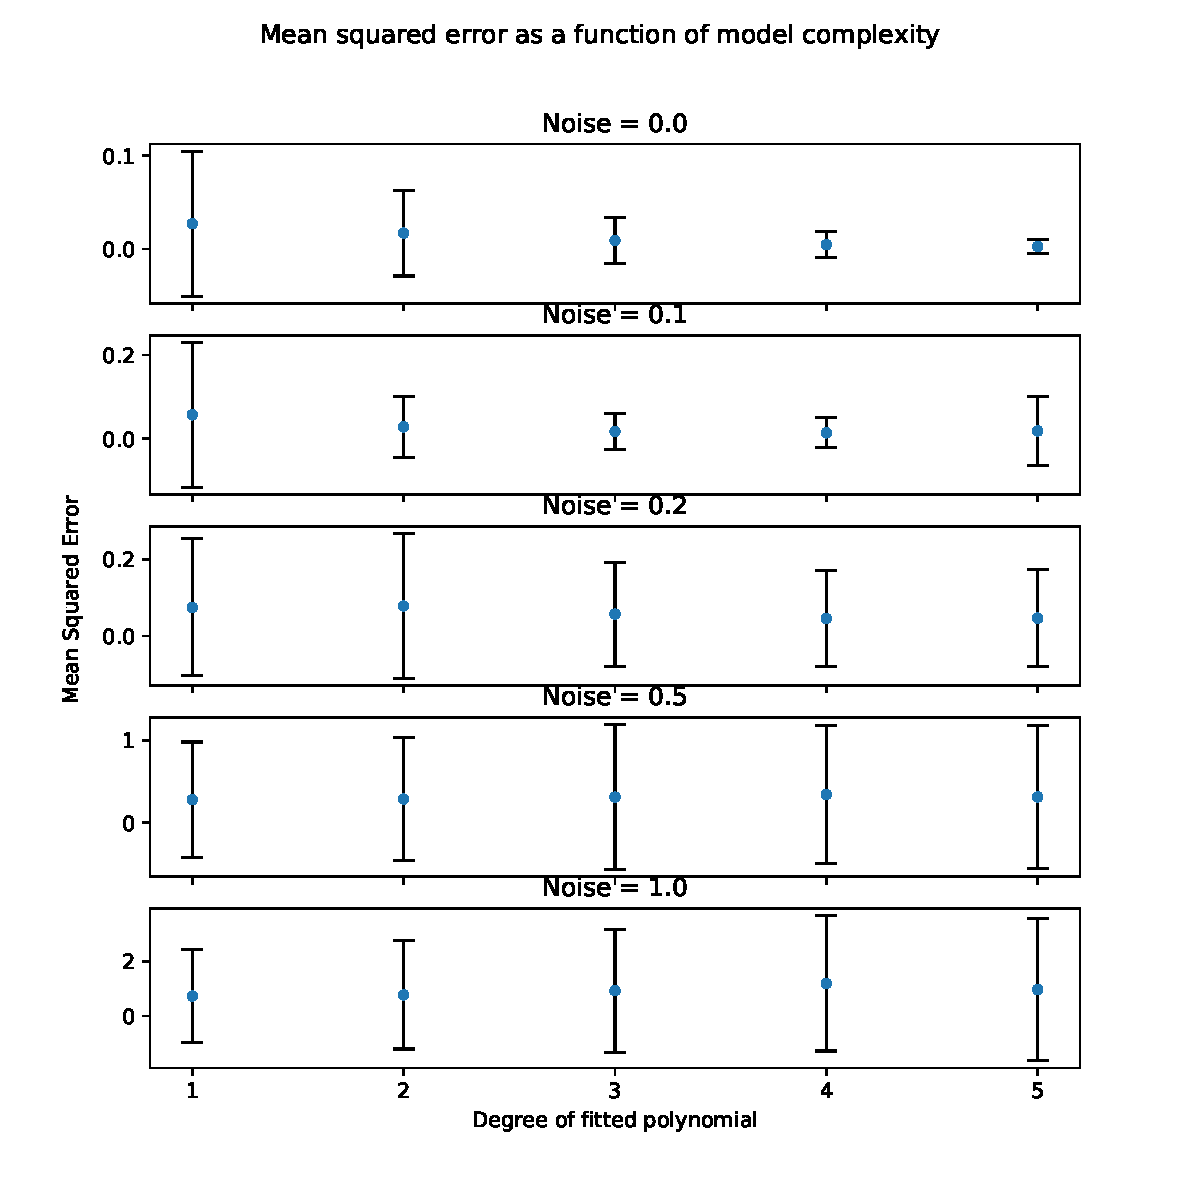
\includegraphics[width = 0.8\paperwidth]{figures/mse_vs_complexity_a.pdf}
    \caption{Plot of Mean Squared Error as a function of model complexity (degree of the
	    fitted polynomial) when fitting with Ordinary Least Squares regression. Each plot
	    from top to bottom shows results for a different degree of stochastic noise added
	    to the training data.}
    \label{fig:ols-mse-complexity}
\end{figure}

\begin{figure}[h]
    %\centering
    %\hspace{-2.8cm}
    \includegraphics[width = 0.8\paperwidth]{figures/r2_vs_complexity_a.pdf}
    \caption{Plot of R2 score as a function of model complexity (degree of the
	    fitted polynomial) when fitting with Ordinary Least Squares regression. Each plot
	    from top to bottom shows results for a different degree of stochastic noise added
	    to the training data.}
    \label{fig:ols-r2-complexity}
\end{figure}

\begin{figure}[h]
    %\centering
    %\hspace{-2.8cm}
    \includegraphics[width = 0.8\paperwidth]{figures/coeffs_vs_complexity_a.pdf}
    \caption{Coefficients for each individual term of the fitted polynomial, after regression. Each
	coefficient is shown with it's confidence interval (95\%), calculated from the variance obtained
	through bootstrapping.}
    \label{fig:ols-coeff-complexity}
\end{figure}

\begin{figure}[h]
    %\centering
    %\hspace{-2.8cm}
    \includegraphics[width = 0.8\paperwidth]{figures/best_coeff_vs_noise_a.pdf}
    \caption{Coefficients for the best polynomial fit based on MSE values. Each plot from top to bottom
	shows the coefficients with their confidence interval (95\%), calculated from the variance obtained
	through bootstrapping, for varying degrees of stochastic noise added to the training data.}
    \label{fig:ols-coeff-noise}
\end{figure}

\begin{figure}[h]
    %\centering
    %\hspace{-2.8cm}
    \includegraphics[width = 0.8\paperwidth]{figures/errors_vs_complexity_a.pdf}
    \caption{In-sample and out-of-sample errors plotted as a function of model complexity (degree of fitted
	polynomial).}
    \label{fig:ols-errors-complexity}
\end{figure}
